\documentclass[10pt, a4paper]{article}

% Packages indispensables
\usepackage[utf8]{inputenc}
\usepackage[T1]{fontenc}
\usepackage[french]{babel}
\usepackage{geometry}
\geometry{margin=2.5cm}
\usepackage{graphicx}
\usepackage{booktabs}
\usepackage[colorlinks=true, linkcolor=black, citecolor=black, urlcolor=blue, pdfborder={0 0 0}]{hyperref}
\usepackage{amsmath}
\usepackage{multicol}
\usepackage{caption}
\usepackage{subcaption}
\usepackage{xcolor}
\usepackage{float}
\usepackage{titlesec}

% chemin des figures
\graphicspath{{../figures}}

% Commandes perso
\newcommand{\bornesup}{$>50K$}
\newcommand{\borneinf}{$\leq50K$}

% Redéfinition des sous-sections
\titleformat{\subsection}[runin]
  {\normalsize\bfseries}{\thesubsection}{1em}{}

% Métadonnées
\title{\textbf{Rapport de modélisation : Prédiction des revenus (Adult Dataset)} \\
\vspace{0.2cm}
       \normalsize Projet Machine Learning --- M2 SDD}
\author{Matthieu PELINGRE}
\date{\today}

\begin{document}

\maketitle

\begin{abstract}
Ce rapport synthétise les travaux de nettoyage, d'exploration et de modélisation effectués sur le jeu de données \textit{Adult}. L'objectif est de prédire si un individu perçoit un revenu annuel supérieur à 50~000~\$ en fonction de caractéristiques socio-démographiques. Le modèle XGBoost optimisé a été retenu comme modèle final, atteignant un F1-macro de 0,8137 et une aire sous la courbe ROC (AUC) de 0,9319, confirmant sa forte capacité de généralisation.
\end{abstract}


% ─────────────────────────────────────────────────────────────────────
\section{Introduction}
L'objectif de ce projet est de prédire si le revenu annuel d'un individu dépasse \textbf{50~000~\$} à partir de données socio-démographiques issues du recensement américain de 1994 (\emph{Adult / Census Income Dataset}, UCI ML Repository~\cite{adult2}). Ce jeu de données contient 48~842 entrées pour 15 variables (14 variables explicatives dont 6 numériques et 8 catégorielles + 1 cible).

Le problème traité est une tâche de classification binaire sur des données tabulaires. La variable cible, \texttt{income}, présente un déséquilibre modéré : environ 24,2~\% des individus appartiennent à la classe minoritaire (\bornesup) contre 75,8~\% pour la classe majoritaire (\borneinf). N'ayant pas de contexte métier, et afin de garantir un compromis optimal entre la Précision (P) et le Rappel (R), la métrique d'évaluation principale retenue pour l'optimisation des modèles et l'évaluation des performances est le \textbf{F1-score (macro)}.


% ─────────────────────────────────────────────────────────────────────
\section{Préparation des données}

Préalablement à toute modélisation ou analyse exploratoire, une phase d'inspection et de nettoyage du jeu de données a été opérée. Cette étape a débuté par la suppression de \texttt{fnlwgt} : poids statistique de pondération, sans valeur prédictive directe.
La variable quantitative \texttt{education} a également été supprimée car redondante avec \texttt{education-num}, correspondant à la même variable, mais encodée selon une échelle ordinale.

L'étape suivante a été l'identification et la gestion des valeurs manquantes. Dans le contexte spécifique de ce registre socio-démographique, une attention particulière a été portée à la détection de caractères de substitution non standards (comme le symbole \textit{?}, employé comme marqueur d'absence) agissant comme des valeurs nulles dissimulées pour les variables \texttt{workclass}, \texttt{occupation} et \texttt{native-country}. Une stratégie de traitement a alors été implémentée pour pallier ce déficit informationnel. Les valeurs manquantes type MNAR (Missing Not At Random), pouvant donc être vectrices d'information, ont été remplacées par une nouvelle modalité \textit{Unknown}. D'autre part, les observations comportant des valeurs manquantes de type MCAR (Missing Completely At Random) ont été exclues afin d'éviter la propagation d'incertitudes.

Enfin, la variable \texttt{native-country} (41 modalités très creuses) a été remplacée par \texttt{native-subregion} regroupant les pays en 10 sous-régions géographiques (standard M49 de l'ONU~\cite{unm49}), réduisant le bruit et la dimensionnalité.

À l'issue de ce protocole, la matrice de données a été jugée structurellement saine et optimale, constituant un socle fiable pour l'analyse exploratoire.


% ─────────────────────────────────────────────────────────────────────
\section{Analyse Exploratoire des Données (EDA)}

L'analyse univariée a permis de dresser le profil statistique des différentes variables. L'examen des variables quantitatives a révélé des distributions fortement asymétriques. Du côté des variables qualitatives, l'analyse des fréquences a mis en évidence la prédominance de certaines modalités, telles que l'appartenance écrasante au secteur privé (\textit{Private} pour la variable \texttt{workclass}) et une surreprésentation des individus identifiés comme de sexe masculin ou caucasiens, reflétant la structure démographique et sociétale de la population active américaine en 1994.


L'analyse bivariée par rapport à la variable cible a mis en évidence des signaux forts au sein des variables explicatives. Le niveau d'éducation (\texttt{education-num}, $\rho$ de Spearman $\approx$ \textbf{0.328}), les gains en capital (\texttt{capital-gain}, $\rho \approx$ 0.277) et l'âge (\texttt{age}, $\rho \approx$ 0.269) discriminent efficacement les hauts revenus, la majorité des individus aisés se situant dans une tranche d'âge mûre et présentant des revenus financiers atypiques (Figure~\ref{fig-num_vs_income}). 
Pour les variables catégorielles, le statut marital (\texttt{marital-status}, V de Cramér $\approx$ \textbf{0.449}), en particulier la modalité \textit{Married-civ-spouse}, présente une des plus fortes corrélations avec la cible. La profession (\texttt{occupation}, V $\approx$ 0.350) est également déterminante (Figure~\ref{fig-cat_vs_income}).

% ---
\begin{figure}[htb]
\centering
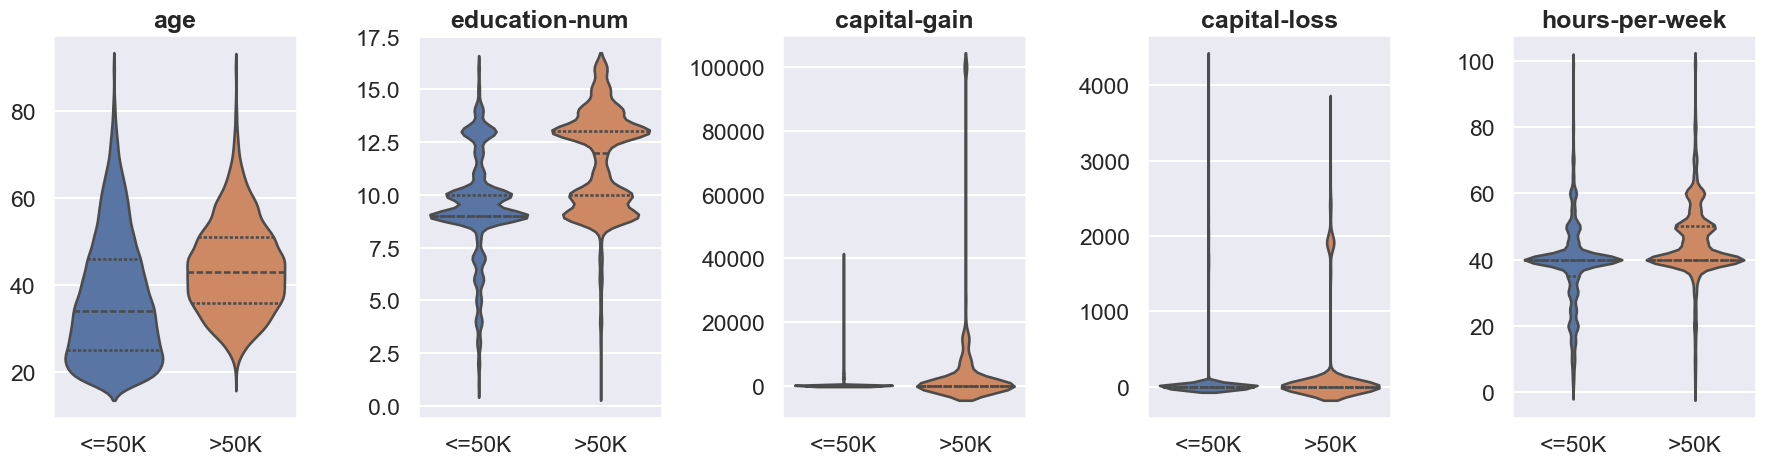
\includegraphics[width=0.8\textwidth]{3-4_violin_num_vs_income.png}
\caption{Distributions des variables numériques par classe de revenu.}
\label{fig-num_vs_income}
\end{figure}


\begin{figure}[htb]
\centering
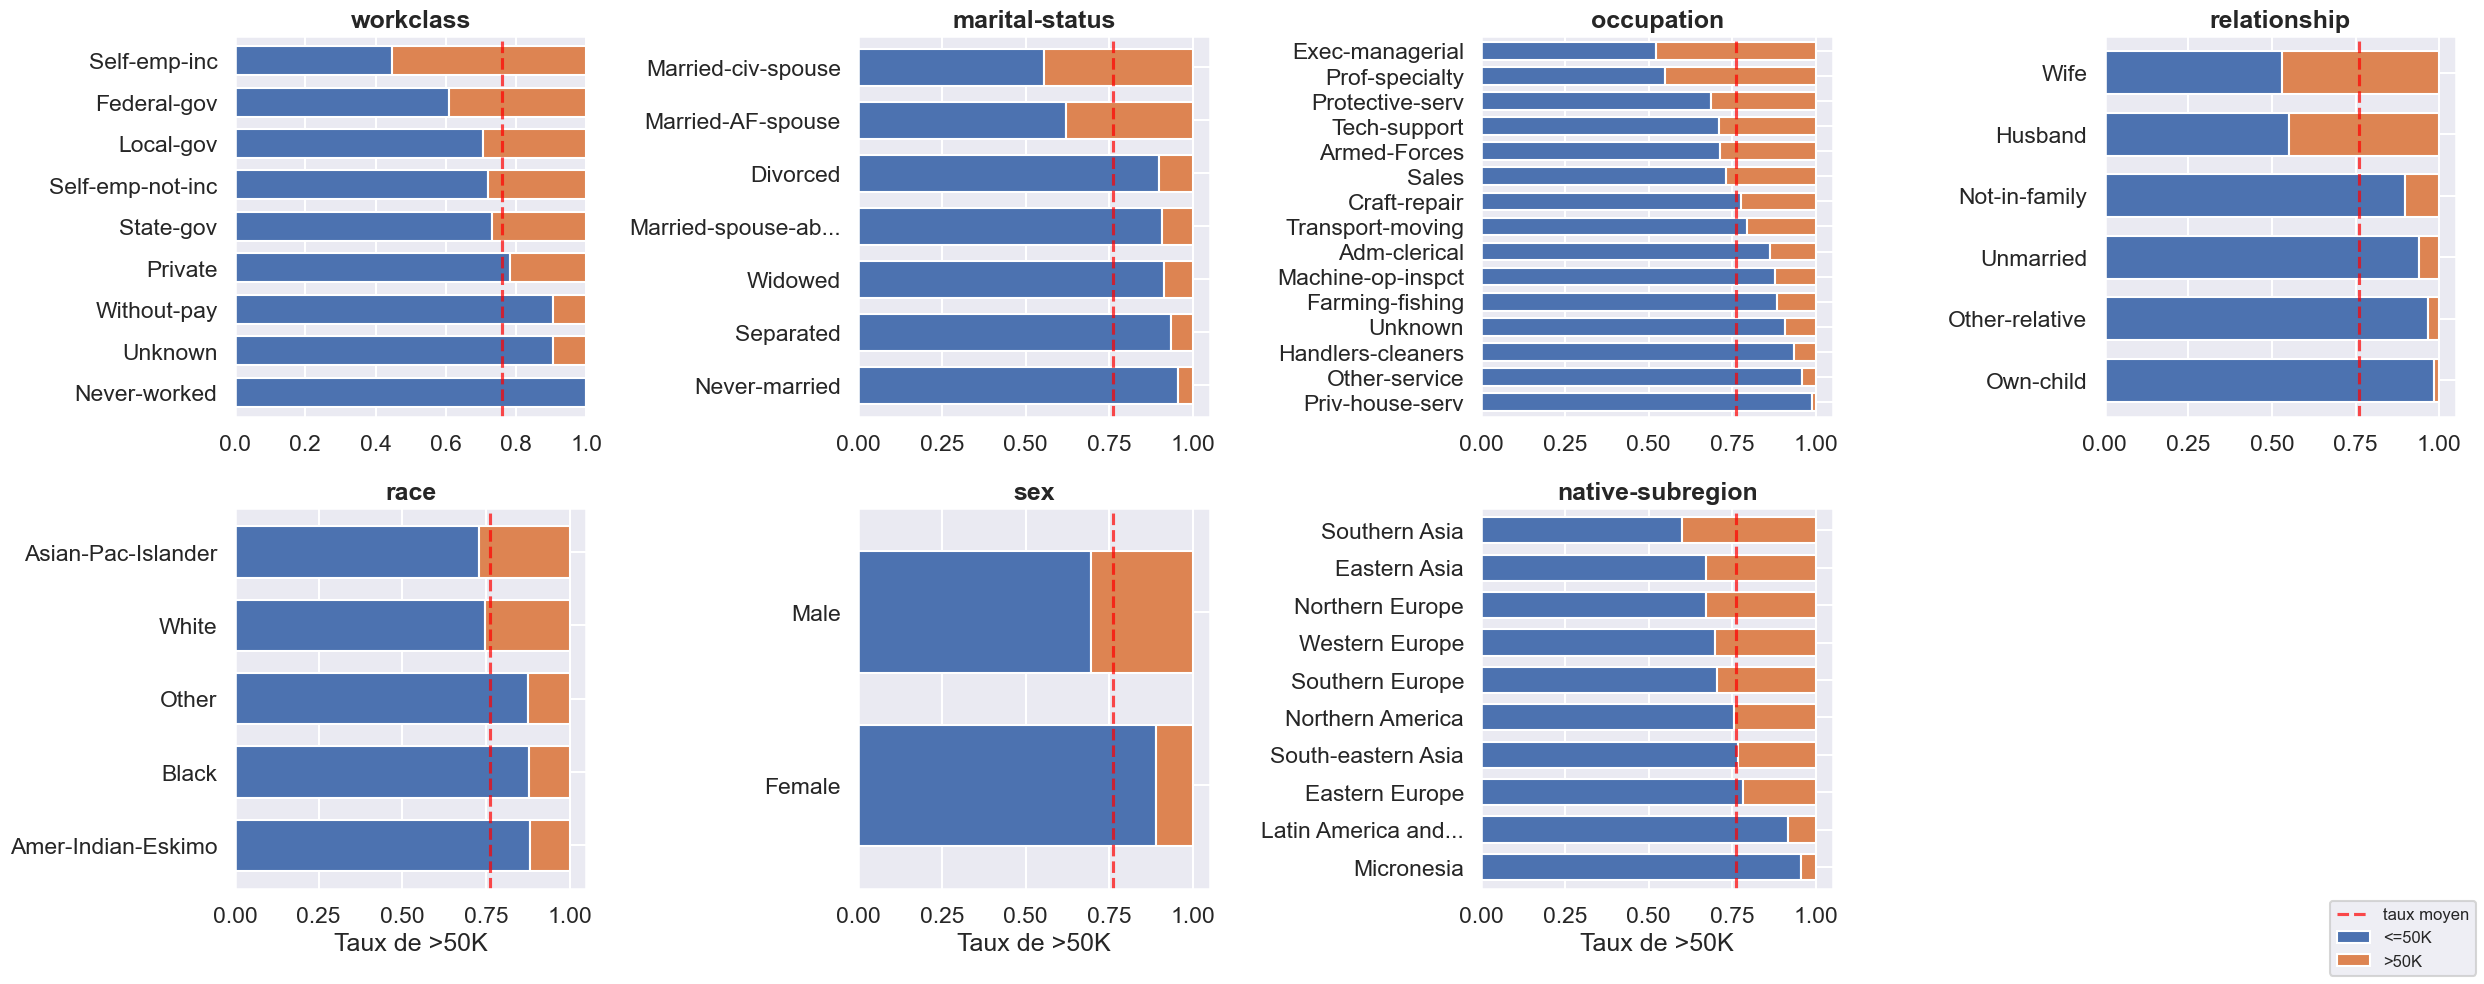
\includegraphics[width=\textwidth]{3-5_stacked_cat_vs_income.png}
\caption{Taux de >50K par modalité.}
\label{fig-cat_vs_income}
\end{figure}

De plus, l'analyse des corrélations entre variables explicatives (Figure~\ref{fig-corr}), ainsi que le calcul de métriques statistiques, telles que l'Information Mutuelle par rapport à la variable cible (Table~\ref{tab-features}), ont permis d'effectuer une sélection des caractéristiques pertinentes, possédant le pouvoir discriminant le plus élevé. En effet, des liens forts, voire de la redondance, peuvent être observés entre \texttt{relationship}, \texttt{sex} et \texttt{marital-status} (Figure~\ref{fig-corr-cramer}). Ces variables partagent globalement des informations similaires. La variable \texttt{relationship} est écartée au profit des variables \texttt{sex} et \texttt{marital-status} afin d'éviter de sur-pondérer ces facteurs au détriment d'autres variables comme l'éducation ou l'âge.


\begin{figure}[htb]
    \centering
    \begin{subfigure}[t]{0.31\textwidth}
        \centering
        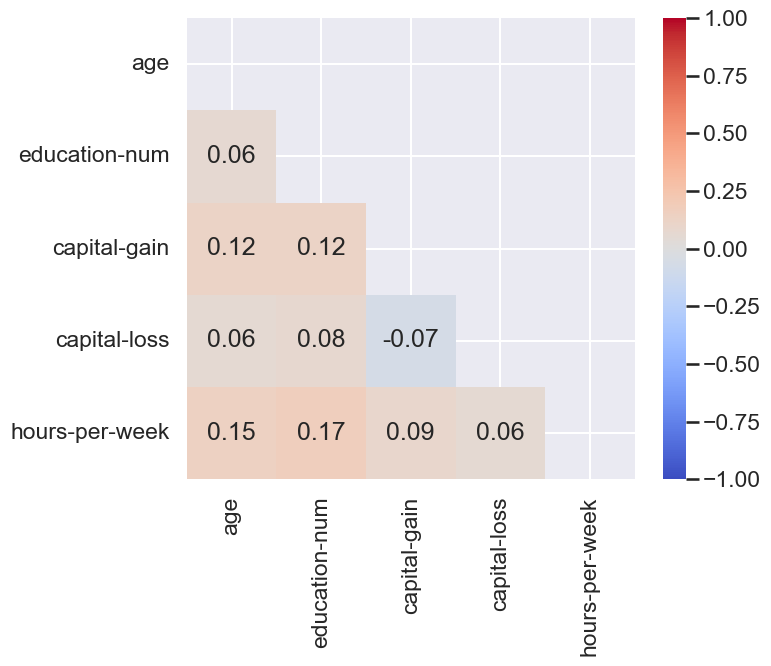
\includegraphics[width=\linewidth]{3-6_correlations_spearman.png}
        \caption{$\rho$ de Spearman}
		\label{fig-corr-spearman}
    \end{subfigure}
    \hfill
    \begin{subfigure}[t]{0.30\textwidth}
        \centering
        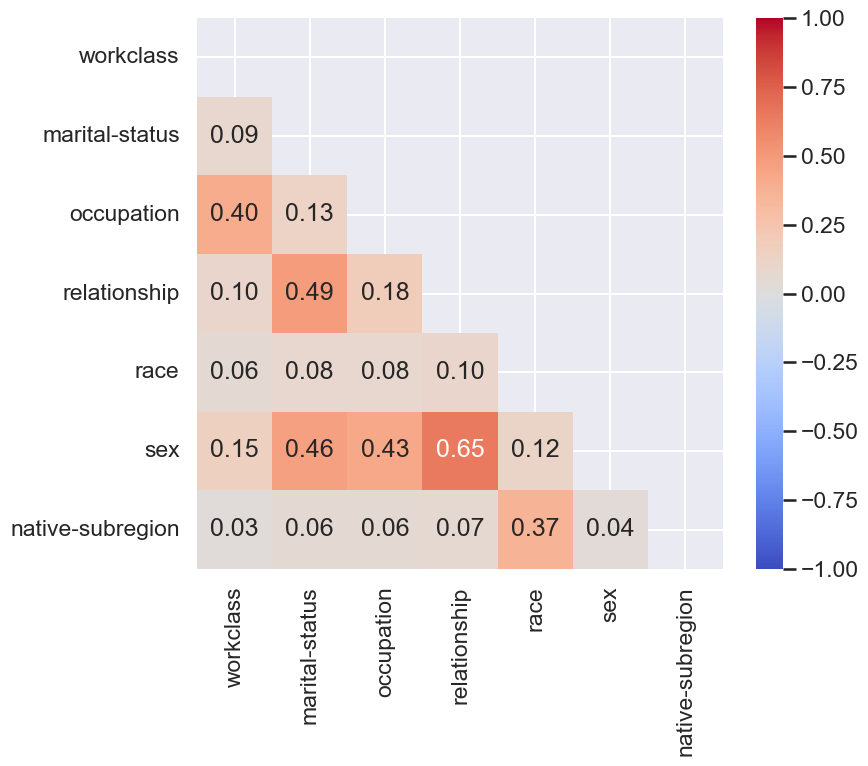
\includegraphics[width=\linewidth]{3-6_correlations_cramer.png}
		\caption{V de Cramér}
		\label{fig-corr-cramer}
    \end{subfigure}
    \hfill
    \begin{subfigure}[t]{0.36\textwidth}
        \centering
        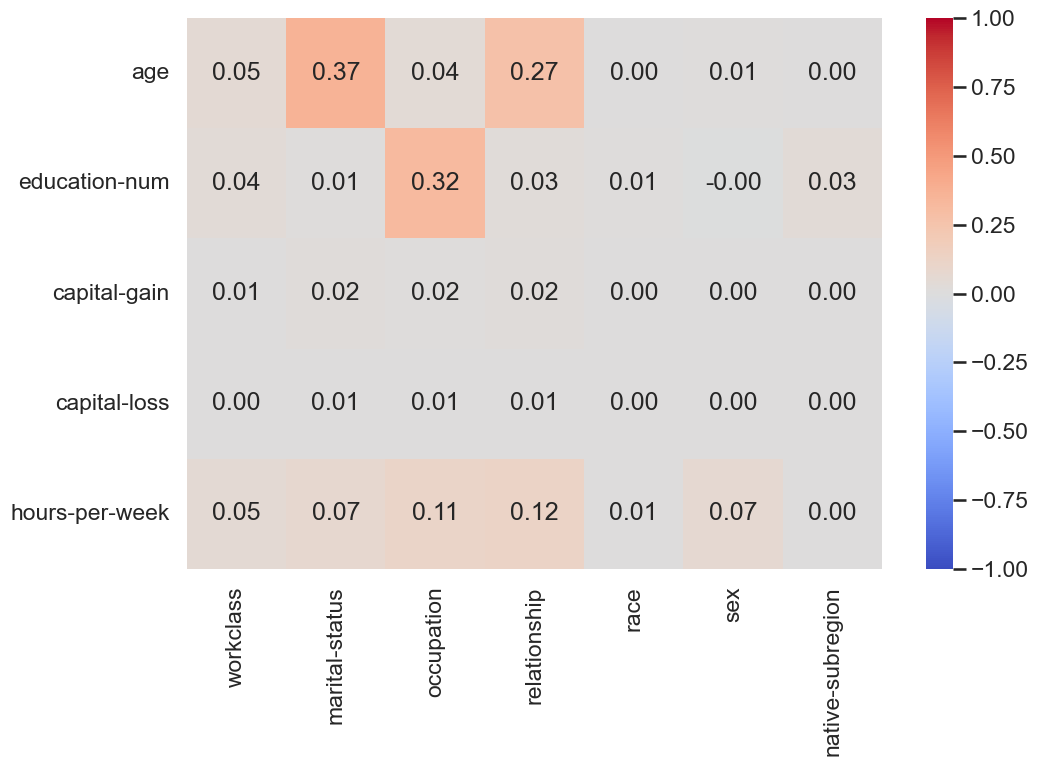
\includegraphics[width=\linewidth]{3-6_correlations_eta.png}
        \caption{$\eta^2$ (Kruskal-Wallis)}
		\label{fig-corr-eta}
    \end{subfigure}
\caption{Analyse des corrélations entre variables explicatives.}
\label{fig-corr}
\end{figure}

Enfin, les variables \texttt{race} (MI $\approx$ 0.006) et \texttt{native-subregion} (MI $\approx$ 0.004), ayant un faible pouvoir discriminant (Table~\ref{tab-features}), sont toutes deux écartées afin de prémunir l'algorithme contre l'assimilation d'un bruit statistique superflu.

\begin{table}[htb]
\centering
\caption{Feature Selection - Pouvoir discriminant des variables par rapport à la variable cible.}
\label{tab-features}
\begin{tabular}{lcccc}
\toprule
 & \textbf{MI} & \textbf{Type} & \textbf{V de Cramér} & \textbf{$\rho$ de Spearman} \\
\midrule
\textbf{\texttt{relationship}}     & \textbf{0.115} & catégorielle & \textbf{0.455} & / \\
\textbf{\texttt{marital-status}}   & \textbf{0.109} & catégorielle & \textbf{0.449} & / \\
\textbf{\texttt{capital-gain}}     & \textbf{0.082} & numérique & / & \textbf{0.277} \\
\texttt{age} & \textbf{0.067}      & numérique & / & 0.269 \\
\textbf{\texttt{education-num}}    & \textbf{0.067} & numérique & / & \textbf{0.328} \\
\textbf{\texttt{occupation}}       & \textbf{0.064} & catégorielle & \textbf{0.350} & / \\
\texttt{hours-per-week}            & 0.040 & numérique & / & 0.269 \\
\texttt{capital-loss}              & 0.036 & numérique & / & 0.138 \\
\texttt{sex}                       & 0.025 & catégorielle & 0.215 & / \\
\texttt{workclass}                 & 0.015 & catégorielle & 0.181 & / \\
\textit{\texttt{race}}             & \textit{0.006} & catégorielle & 0.100 & / \\
\textit{\texttt{native-subregion}} & \textit{0.004} & catégorielle & 0.087 & / \\
\bottomrule
\end{tabular}
\end{table}

% ─────────────────────────────────────────────────────────────────────
\section{Méthodologie}

\subsection*{Prétraitements.} 
Afin d'éviter toute fuite de données (\textit{Data Leakage}) lors de la validation croisée, les étapes de transformation ont été rigoureusement encapsulées dans des \texttt{Pipeline} Scikit-Learn. Les variables numériques sont normalisées et les variables catégorielles encodées en vecteurs One-Hot.

\subsection*{Évaluation des baselines.}
Une analyse des baselines disponibles sur le dépôt UCI ML~\cite{adult2}, couplées aux observations de l'EDA, a permis d'écarter la Régression Logistique, les SVM et les Réseaux de Neurones. Les modèles basés sur les arbres (Random Forest et XGBoost), plus appropriés pour des données tabulaires contenant des variables numériques fortement asymétriques comme dans ce jeu de données, se démarquent avec des Exactitudes (Acc) et Précisions (P) de :
\begin{itemize}
\item Random Forest : 0.834 $\pm$ 0.08 (Acc) et 0.802 $\pm$ 0.09 (P)
\item XGBoost : 0.872 $\pm$ 0.05 (Acc) et 0.834 $\pm$ 0.08 (P)
\end{itemize}

\noindent Trois modèles ont donc été entraînés et comparés : \emph{DummyClassifier}, Random Forest~\cite{randomforest} et XGBoost~\cite{xgboost}. 

\subsection*{Métrique d'optimisation.}
Le \textbf{F1-score macro} a été retenu comme métrique principale. En effet, étant la moyenne harmonique entre Précision et Rappel, il équilibre ces métriques sur les deux classes sans nécessiter d'hypothèse métier sur le coût relatif des erreurs.

\subsection*{Optimisation des hyperparamètres.}
Une optimisation par \texttt{RandomizedSearchCV} a été menée sur Random Forest et XGBoost. Un point d'attention particulier a été porté sur la gestion du déséquilibre des classes en intégrant les paramètres \texttt{class\_weight} et \texttt{scale\_pos\_weight} dans l'espace de recherche. 


% ─────────────────────────────────────────────────────────────────────
\section{Résultats \& Discussion}

De manière intéressante, les algorithmes ont convergé vers des modèles n'utilisant \textbf{aucune pondération artificielle}. L'optimisation basée sur le F1-score a prouvé que sacrifier massivement la Précision pour augmenter le Rappel (via les poids) détériorait la performance globale. Les modèles ont compensé ce déséquilibre par des choix structurels (ex: des arbres profonds mais élagués pour le Random Forest, et de nombreux arbres de faible profondeur avec un faible \texttt{learning\_rate} pour XGBoost).

\medskip
\noindent\textbf{Meilleurs hyperparamètres :}\\
\begin{minipage}[t]{0.48\textwidth}
    \noindent Random Forest (F1-macro CV = 0.799) : \\
    \begin{tabular}{ll}
    --- \texttt{n\_estimators}       & = 584, \\
    --- \texttt{max\_depth}          & = 20, \\
    --- \texttt{min\_samples\_split} & = 4, \\
    --- \texttt{min\_samples\_leaf}  & = 4, \\
    --- \texttt{max\_features}       & = \textit{None}, \\
    --- \texttt{class\_weight}       & = \textit{None} \\
	\end{tabular}
\end{minipage}
\hfill
\begin{minipage}[t]{0.48\textwidth}
    \noindent XGBoost (F1-macro CV = 0.816) : \\
	\begin{tabular}{ll}
	--- \texttt{n\_estimators}       & = 922, \\
	--- \texttt{max\_depth}          & = 5, \\
	--- \texttt{learning\_rate}      & = 0.04, \\
	--- \texttt{subsample}           & = 0.99, \\
	--- \texttt{colsample\_bytree}   & = 0.94, \\
	--- \texttt{gamma}               & = 0.10, \\
	--- \texttt{reg\_lambda}         & = 0.69, \\
	--- \texttt{scale\_pos\_weight}  & = 1 \\
	\end{tabular}
\end{minipage}

\medskip

\noindent\textit{Note : les poids de classes n'ont pas amélioré le F1-macro malgré le déséquilibre 3:1 --- les arbres ensemblistes gèrent naturellement ce déséquilibre modéré.}

\medskip

Les modèles optimisés ont ensuite été évalués sur le même ensemble de test, ensemble indépendant des données utilisées lors de la validation croisée (CV). Le tableau \ref{tab-resultats} résume les performances obtenues.

\begin{table}[htb]
\centering
\caption{Comparaison des modèles sur l'ensemble de test}
\label{tab-resultats}
\begin{tabular}{lccccc}
\toprule
\textbf{Modèle} & \textbf{Acc} & \textbf{P} & \textbf{R} & \textbf{F1-macro} & \textbf{AUC-ROC} \\
\midrule
DummyClassifier          & 0.753 & 0.376 & 0.500 & 0.429 & 0.500 \\
Random Forest            & 0.862 & 0.833 & 0.775 & 0.798 & 0.920 \\
\textbf{XGBoost}         & \textbf{0.871} & \textbf{0.843} & \textbf{0.794} & \textbf{0.814} & \textbf{0.932} \\
\bottomrule
\end{tabular}
\end{table}

Notre méthodologie a prouvé son efficacité en permettant au modèle Random Forest de surpasser largement sa baseline initiale.
Le modèle \textbf{XGBoost}, lui, devance le Random Forest sur l'ensemble des métriques. Sa Précision dépasse de peu celle de sa très solide \textit{baseline}, mais sa capacité de séparation des classes est validée par un AUC-ROC remarquable de 0,932 (Figure~\ref{fig-test-roc}).

Par ailleurs, la similitude observée entre les performances issues de la validation croisée (CV) lors de la phase d'optimisation et celles obtenues sur l'ensemble de test indépendant valide la robustesse de notre méthodologie. Cette stabilité des métriques, notamment du F1-score (pour XGBoost : 0.816 en CV contre 0.814 sur l'ensemble de test), atteste d'une excellente capacité de généralisation des algorithmes retenus et permet d'écarter toute suspicion de sur-apprentissage (\textit{overfitting}). Elle confirme l'efficacité des hyperparamètres de régularisation sélectionnés et garantit la fiabilité du modèle pour des inférences futures sur des données inédites.

\begin{figure}[htb]
    \centering
    \begin{subfigure}[t]{0.45\textwidth}
        \centering
        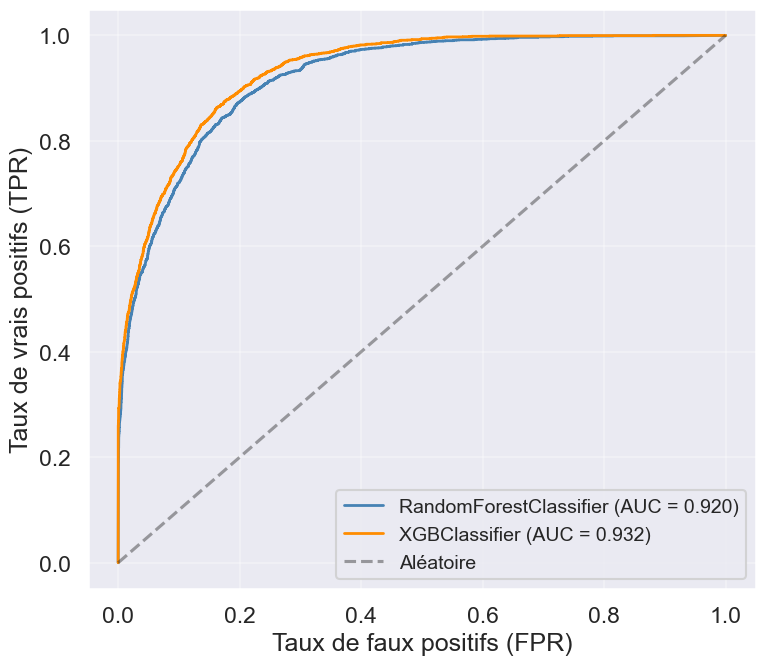
\includegraphics[width=\linewidth]{4-5_models_comparison_roc.png}
        \caption{Courbes ROC des modèles optimisés.}
        \label{fig-test-roc}
    \end{subfigure}
    \hfill
    \begin{subfigure}[t]{0.53\textwidth}
        \centering
        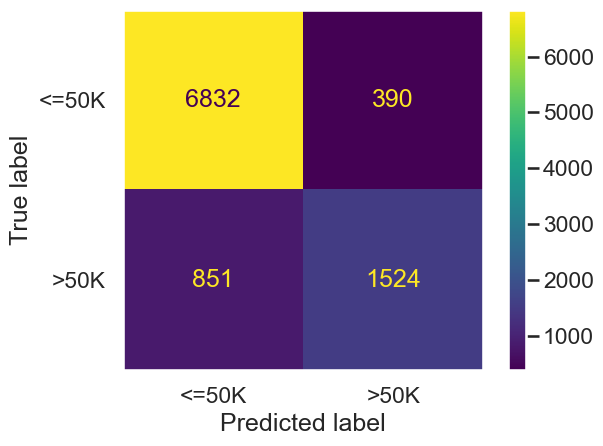
\includegraphics[width=\linewidth]{4-4_xgb_confusion_matrix.png}
        \caption{Matrice de confusion --- XGBoost.}
        \label{fig-test-xgboost}
    \end{subfigure}
    \caption{Résultats obtenus sur l'ensemble de test indépendant.}
    \label{fig-test}
\end{figure}


% ─────────────────────────────────────────────────────────────────────
\section{Interprétabilité}
L'analyse des importances des caractéristiques extraites du modèle XGBoost (Figure~\ref{fig-feat-importance}) met en exergue la prédominance absolue du statut marital dans le processus décisionnel de l'algorithme. À elles seules, les modalités \textit{Married-civ-spouse} (36,9 \%) et \textit{Never-married} (7,8 \%) concentrent environ 45 \% du poids prédictif global. Les gains en capital (\texttt{capital-gain}), représentant 6,7 \% de l'importance mathématique, s'affirment comme un proxy robuste des investissements financiers. Enfin, le niveau d'éducation formelle (\texttt{education-num}, pesant pour 5,1 \%) et la profession, dont plusieurs modalités se hissent parmi les quinze descripteurs les plus influents, complètent ce profilage socio-économique en confirmant leur rôle déterminant dans la discrimination des hauts revenus. Les importances des caractéristiques obtenues corroborent ainsi les hypothèses dégagées lors de l'analyse exploratoire.

Le déploiement du modèle a également été simulé, à l'aide du \texttt{Pipeline} Scikit-learn exporté au format \texttt{joblib}.
Pour garantir également la transparence du modèle sélectionné en production, l'approche \textbf{SHAP}~\cite{shap} (SHapley Additive exPlanations) a été implémentée, à l'aide d'un \texttt{TreeExplainer}. En extrayant les noms des variables post-encodage, les graphiques en cascade (\textit{Waterfall plots}) ont permis de vérifier le comportement local de l'algorithme (Figure~\ref{fig-shap}). 

\begin{figure}[htb]
    \centering
    \begin{subfigure}[t]{0.49\textwidth}
        \centering
        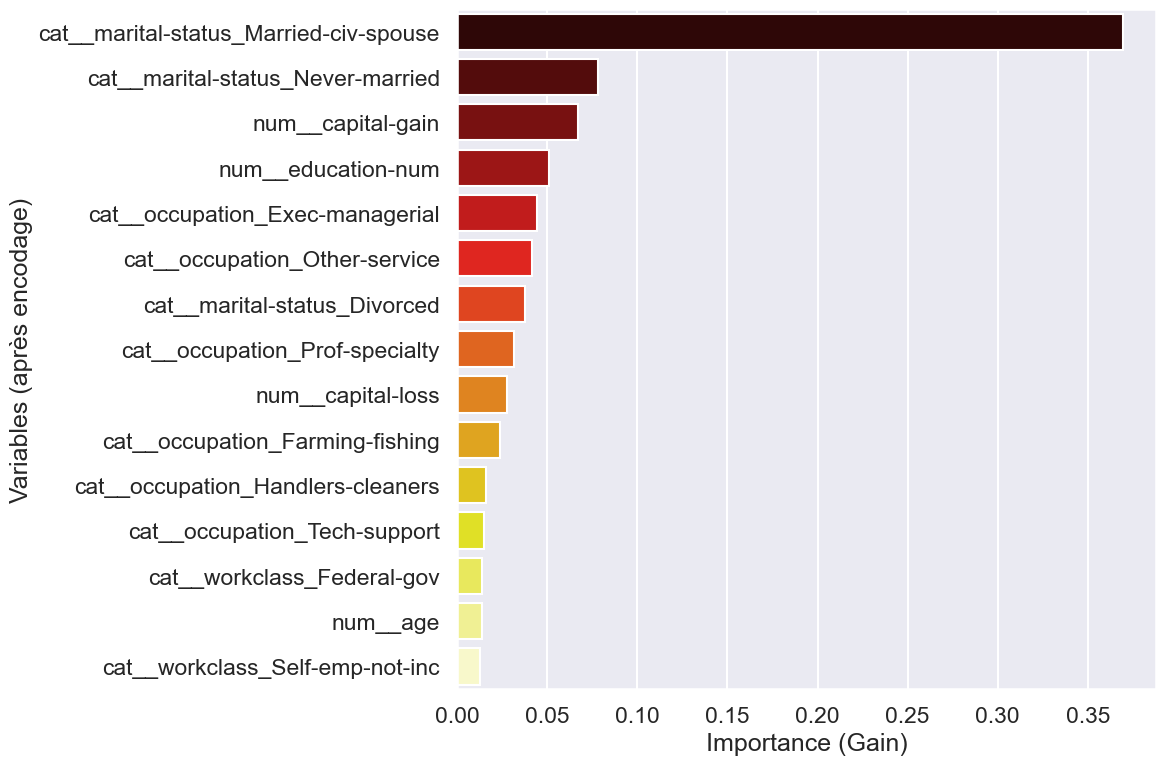
\includegraphics[width=\linewidth]{5_feature_importance.png}
        \caption{Top 15 des importance des caractéristiques (global).}
        \label{fig-feat-importance}
    \end{subfigure}
    \hfill
    \begin{subfigure}[t]{0.49\textwidth}
        \centering
        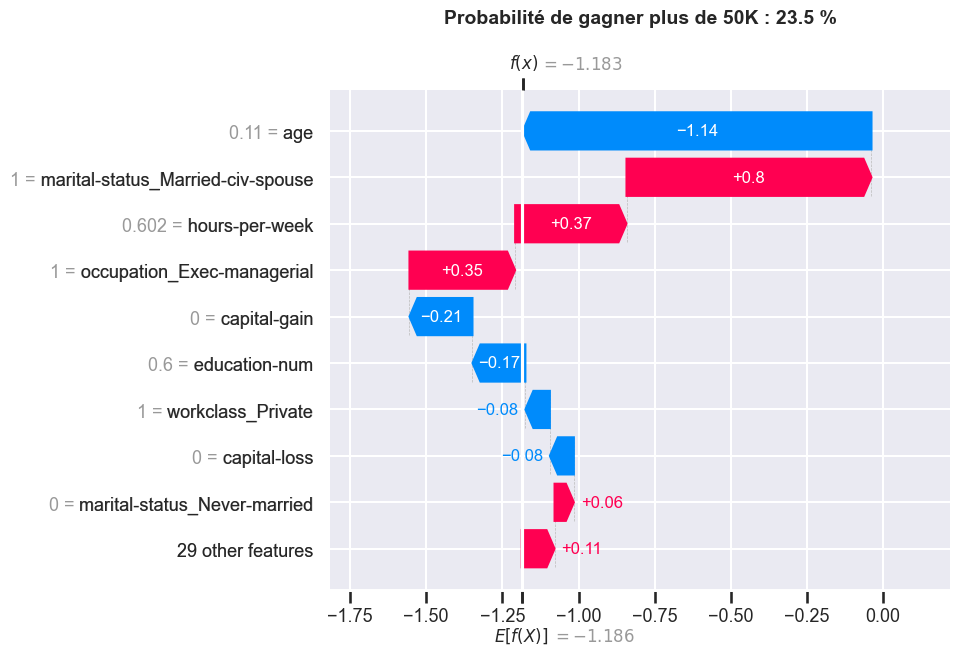
\includegraphics[width=\linewidth]{7_SHAP.png}
        \caption{Valeurs SHAP pour un individu exemple (local).}
        \label{fig-shap}
    \end{subfigure}
    \caption{Interprétabilité globale et locale du modèle XGBoost obtenu.}
    \label{fig-xai}
\end{figure}


% ─────────────────────────────────────────────────────────────────────
\section{Conclusion}
Ce projet a mis en œuvre un pipeline de \textit{Machine Learning} complet, robuste et transparent, sur le dataset Adult Census. 
L'analyse exploratoire préliminaire a mis en évidence que le \textbf{statut marital} et le \textbf{capital financier} sont les déterminants dominants du revenu, tandis que l'origine géographique et la race ont un impact marginal. 

XGBoost s'est révélé être l'algorithme le plus adapté à ces données tabulaires. La haute qualité de l'ingénierie des caractéristiques (\textit{Feature Engineering}) a permis d'obtenir d'excellentes prédictions sans recourir à des méthodes de sur-échantillonnage complexes comme SMOTE~\cite{smote}.

Enfin, l'implémentation SHAP en production garantit l'explicabilité des décisions, un prérequis essentiel pour tout déploiement responsable.


% ---- Bibliography ----
\newpage
\bibliographystyle{splncs04}
\bibliography{references}

\end{document}
